%\documentclass[a4paper,12pt]{report}
\documentclass[a4paper,12pt]{article}
%\documentclass[a4paper,12pt]{book}
\usepackage{polski}
\usepackage[polish]{babel}
\usepackage[utf8]{inputenc}
\usepackage[top=2.5cm, bottom=2.5cm, left=3cm, right=2.5cm]{geometry}
\usepackage{graphicx}
\usepackage{setspace}
\usepackage{ifthen}
%\usepackage[utf8]{inputenc}
\usepackage{a4wide}
\usepackage{fullpage}
\usepackage{verbatim}
\usepackage[usenames,dvipsnames]{xcolor}
\usepackage{hyperref}
\usepackage{subfig}
\usepackage{listings}
\usepackage{mdwlist}
\usepackage{titlesec}
\usepackage{lipsum}
\usepackage{tikz}
\usetikzlibrary{positioning,shapes,shadows,arrows}
\definecolor{uwaga}{HTML}{E59C9C}

\hypersetup{
	bookmarks=true,
	pdftitle={GasAnalyzer},
	pdfauthor={Damian Karbowiak, Grzegorz Powała},
	pdfsubject={GasAnalyzer},
	pdfkeywords={GasAnalyzer, Siemens, przemysł, przemysłówka, ppsk},
	colorlinks=true,
	linkcolor=Blue,
	urlcolor=Blue
	}

\let\subsubsubsection\paragraph
%\setcounter{secnumdepth}{6} % subsubparagraph ???
% that is, subsubsubsubsubsection :-)
\setcounter{secnumdepth}{4}

%\titlespacing{\section}{1cm}{*4}{*1.5}
%\titlespacing{\subsection}{1cm}{*4}{*1.5}
%\titlespacing{\subsubsection}{1cm}{*4}{*1.5}

\def\tytul{Gas Analyzer}
\def\przedmiot{Projektowanie przemysłowych systemów komputerowych}
\def\autor{Autorzy: Damian Karbowiak, Grzegorz Powała}
\def\sem{Informatyka, SSM3, grupa ISP1}
\def\prow{Prowadzący: dr inż. Jacek Stój}
\def\kons{Konsultant: mgr inż. Tomasz Kress}

\begin{document}
\tikzstyle{abstract}=[rectangle, draw=black, rounded corners, fill=blue!40, drop shadow,
        text centered, anchor=north, text=white, text width=3cm]
\tikzstyle{comment}=[rectangle, draw=black, rounded corners, fill=green, drop shadow,
        text centered, anchor=north, text=white, text width=3cm]
\tikzstyle{myarrow}=[->, >=open triangle 90, thick]
\tikzstyle{line}=[-, thick]
\lstset{backgroundcolor=\color{white}, boxpos=c, captionpos=b}
\lstset{numbers=left, stepnumber=1, numbersep=10pt, frame=single}
\lstset{frameround=tttt}
\renewcommand{\lstlistlistingname}{\vspace*{-13mm}}
\renewcommand{\listfigurename}{\vspace*{-13mm}}
%\renewcommand*\l@figure[2]{\indent}
\renewcommand{\listtablename}{\vspace*{-13mm}}
\renewcommand*{\refname}{\vspace*{-13mm}}
\renewcommand{\lstlistingname}{Kod źródłowy} 
%\documentclass[a4paper,12pt]{report}
\documentclass[a4paper,12pt]{article}
%\documentclass[a4paper,12pt]{book}
\usepackage{polski}
\usepackage[polish]{babel}
\usepackage[utf8]{inputenc}
\usepackage[top=2.5cm, bottom=2.5cm, left=3cm, right=2.5cm]{geometry}
\usepackage{graphicx}
\usepackage{setspace}
\usepackage{ifthen}
%\usepackage[utf8]{inputenc}
\usepackage{a4wide}
\usepackage{fullpage}
\usepackage{verbatim}
\usepackage[usenames,dvipsnames]{color}
\usepackage{hyperref}
\usepackage{subfig}
\usepackage{listings}
\usepackage{mdwlist}
\usepackage{titlesec}
\usepackage{lipsum}

\hypersetup{
	bookmarks=true,
	pdftitle={Zdalne laboratorium},
	pdfauthor={Damian Karbowiak},
	pdfsubject={Zdalne laboratorium},
	pdfkeywords={Zdalny, laboratorium, przemysł, przemysłówka, psp, sip},
	colorlinks=true,
	linkcolor=Blue,
	urlcolor=Blue
	}

\let\subsubsubsection\paragraph
%\setcounter{secnumdepth}{6} % subsubparagraph ???
% that is, subsubsubsubsubsection :-)
\setcounter{secnumdepth}{4}

\titlespacing{\section}{1cm}{*4}{*1.5}
\titlespacing{\subsection}{1cm}{*4}{*1.5}
\titlespacing{\subsubsection}{1cm}{*4}{*1.5}

\begin{document}
\lstset{backgroundcolor=\color{white}, boxpos=c, captionpos=b}
\lstset{numbers=left, stepnumber=1, numbersep=10pt, frame=single}
\lstset{frameround=tttt}
\renewcommand{\lstlistlistingname}{\vspace*{-13mm}}
\renewcommand{\listfigurename}{\vspace*{-13mm}}
%\renewcommand*\l@figure[2]{\indent}
\renewcommand{\listtablename}{\vspace*{-13mm}}
\renewcommand*{\refname}{\vspace*{-13mm}}
\renewcommand{\lstlistingname}{Kod źródłowy} 

XYZ

\end{document}


\tableofcontents 
\addtocontents{toc}{\protect\vspace*{\baselineskip}}
\clearpage

\section{Wstęp}
%Część ta~zawiera wstępne informacje o~realizowanym projekcie. Zebrano w~nim wszystko to~co było dostępne zanim student przystąpił do~realizacji informatycznej części projektu. Opisano stanowisko laboratoryjne na~którym powstał projekt.

\subsection{Geneza}
Tematem projektu, którego dotyczy to~sprawozdanie jest: Gas Analyzer". Pomysł na~projekt pojawił~się w~wyniku nawiązania przez nas współpracy z~Zakładem Kotłów i Wytwornic Pary, a~dokładnie Panem Tomaszem Kressem.

\subsection{Temat}
Głównymi celami pracy było napisanie oprogramowania umożliwiającego gromadzenie danych pomiarowych z~kilku urządzeń firmy Siemens.

\subsection{Stanowisko}
W~czasie realizacji projektu wykorzystywaliśmy 2~różne stanowiska. W~pierwszej fazie projektu korzystaliśmy z~uproszczonego stanowiska, które wyglądało jak na~Rysunku~\ref{schemat1}. W~dalszej fazie projektu, kiedy mieliśmy już przygotowaną i~przetestowaną wersję podstawową współpracującą z~jednym urządzeniem pomiarowym rozpoczęliśmy pracę na stanowisku docelowym składającym się z~4 urządzeń, które wyglądało jak na Rysunku~\ref{schemat2}.
\subsubsection{Stanowisko prototypowe}
\begin{figure}[!htb] 	\centering 	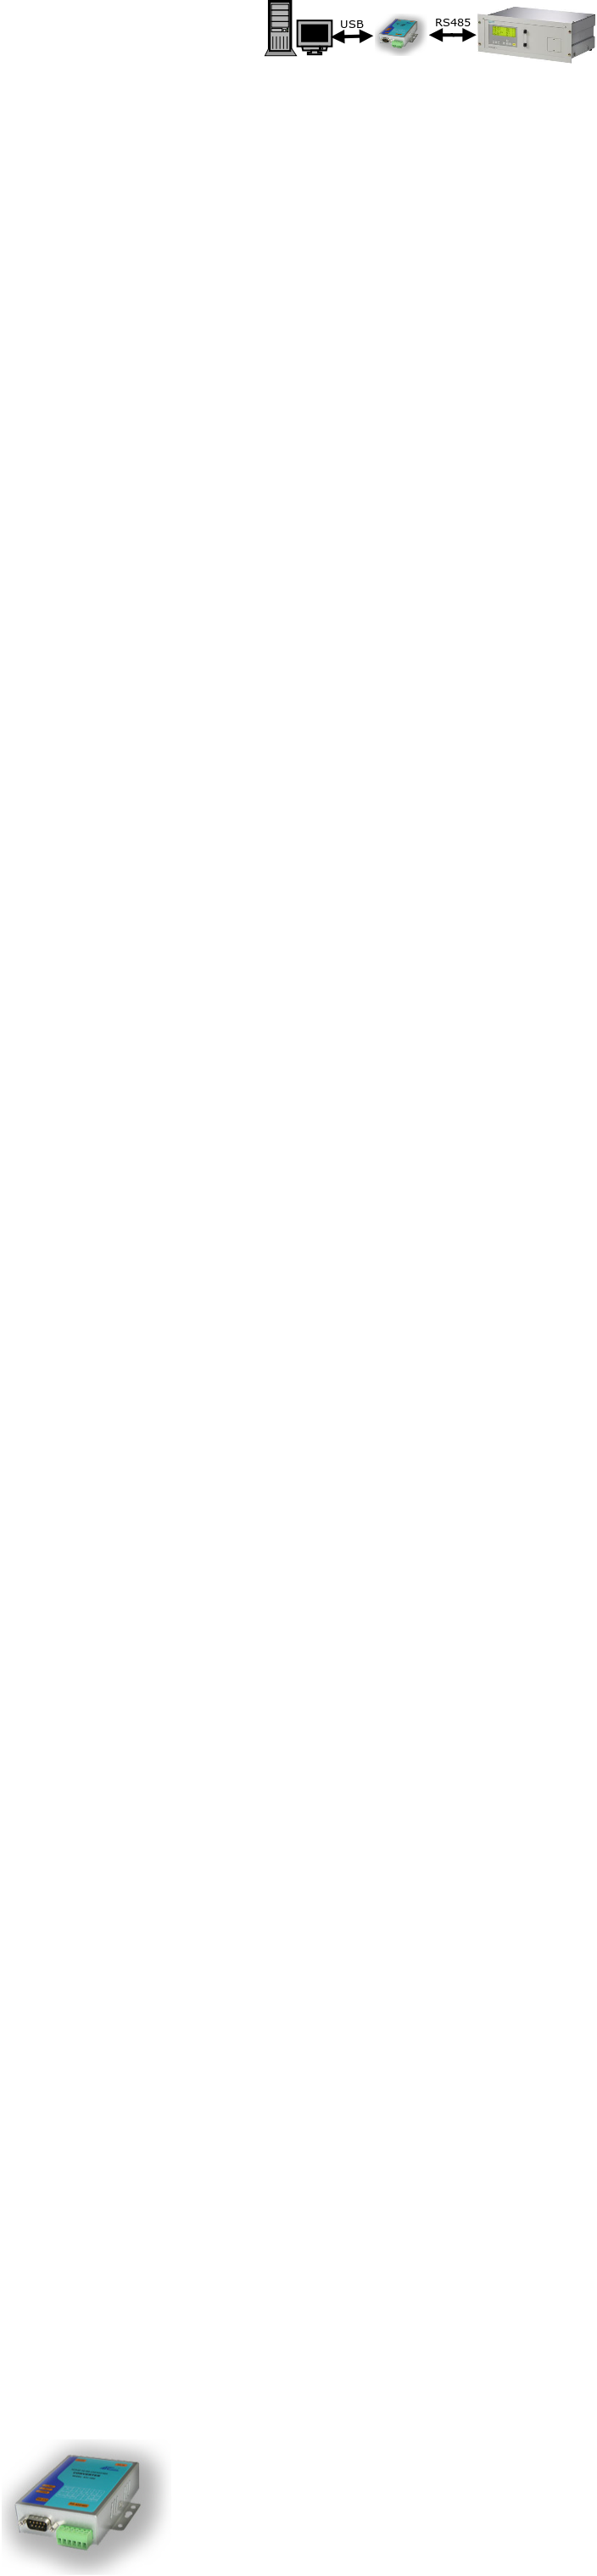
\includegraphics[width=0.8\textwidth]{images/schemat1} 	\caption{Schemat stanowiska prototypowego} \label{schemat1} \end{figure} 
Na~potrzeby realizacji projektu stworzono stanowisko laboratoryjne, którego schemat przedstawia Rysunek~\ref{schemat1}. Składa się ono~z:
\begin{itemize}
\item Komputera,
\item Konwertera ATC-850,
\item ULTRAMAT 23.
\end{itemize}
\indent
\indent Komputery na, których powstała wersja rozwojowa projekty pracowały na systemach operacyjnych Linux Ubuntu w~wersji 32 oraz 64~bitowej. Do~połączenia komputera z~urządzeniem ULTRAMAT~23 zastosowano izolowany konwerter~USB do~RS-232/422/485, moduł ATC-850 jest automatycznie wykrywany i~instalowany jako standardowy port~COM. Stosowane w~tej fazie projektu urządzenie pomiarowe potrafiło mierzyć zawartość $ CO_2 $, $ CO $, $ O_2 $ oraz $ NO_2 $ ??

\subsubsection{Stanowisko docelowe}
\begin{figure}[!htb] 	\centering 	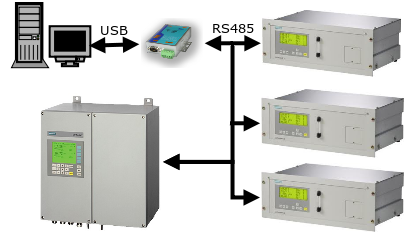
\includegraphics[width=0.8\textwidth]{images/schemat2} 	\caption{Schemat stanowiska docelowego} \label{schemat2} \end{figure} 
Docelowo zrealizowany projekt ma być uruchamiany na~stanowisku, którego schemat przedstawia Rysunek~\ref{schemat2}. Składa się ono~z:
\begin{itemize}
\item Komputera,
\item Konwertera ATC-850,
\item 3x ULTRAMAT 23,
\item ULTRAMAT 6.
\end{itemize}
\indent
\indent Stanowisko docelowe różni się od stanowiska prototypowego po pierwsze systemem operacyjnym, który pracuje na komputerze i jest to Windows XP. Po drugie stanowisko docelowe posiada więcej urządzeń pomiarowych, a jest ich dokładnie cztery i mierzą wartości przedstawione w Tabeli~\ref{tab:docelowe}.

\begin{table}[h]
\centering
\begin{tabular}{|l|l|}
\hline Urządzenie & Wielkości mierzone \\ 
\hline ULTRAMAT~6 & $ NH_3 [vpm] $ \\ 
\hline ULTRAMAT~23 & $ CH_4 [\%], CO [\%], CO_2 [\%], O_2 [\%] $ \\ 
\hline ULTRAMAT~23 & $  $ \\ 
\hline ULTRAMAT~23 & $  $ \\ 
\hline 
\end{tabular} 
\caption{Urządzenia docelowe wraz z wartościami mierzonymi}
\label{tab:docelowe}
\end{table}

\subsection{Analiza tematu}
Analiza tematu polegała przede wszystkim na zapoznaniu się z~narzędziami programistycznymi do~tworzenia oprogramowania sterownika oraz wizualizacji.
Poznanie tych podstaw pozwoliło dobrać język odpowiedni do~realizacji poszczególnych zadań.

\subsection{Założenia}
%Stworzone oprogramowanie dla Robota Fishertechnik ma działać na sterownikach firmy Siemens oraz ma zostać stworzone przy użyciu środowiska Step 7. Funkcjonalności robota, jakie mają wchodzić w~skład projektu, to:
Oprogramowanie do zbierania danych pomiarowych powinno zostać stworzone przy użyciu technologii pozwalającej działać na~różnych systemach operacyjnych bez~skomplikowanych zabiegów.Funkcjonalności wchodzące w~skład projektu,~to:
\begin{itemize}
\item wizualizacja bieżących pomiarów,
\item generowanie raportu z pomiaru jako plik arkusza kalkulacyjnego,
\item generowanie raportu z pomiaru jako plik do wydruku z wynikami np. format~PDF,
\item .
\end{itemize}
\indent
\indent Powyżej zostały wymienione założenia podstawowe, jednak autorzy nie~wykluczają zrealizowania dodatkowych zadań, które nie~zostały zamieszczone w~pierwotnej koncepcji realizacji projektu.

\subsection{Plan pracy}
Realizacja projektu została podzielona na następujące etapy:
\begin{itemize}
\item Przygotowanie stanowiska, zebranie odpowiednich materiałów i~literatury,
\item Analiza wymagań funkcjonalnych aplikacji,
\item Projektowanie struktury oprogramowania i~interfejsów wymiany danych,
\item Implementacja,
\item Testowanie i~uruchamianie,
\item Przedstawienie projektu i~ewentualne korekty.
\end{itemize}
\indent
\indent Powyższy plan pracy stanowił dla autorów wyznacznik kolejnych działań. Jednak powszechnie wiadomo, że w~praktyce poszczególne punkty są~wymienne i~wpływają na siebie wzajemnie.

\begin{table}[h]
\centering
\begin{tabular}{|p{0.15\textwidth}|p{0.15\textwidth}|p{0.7\textwidth}|}
\hline \textbf{Termin} & \textbf{Osoba} & \textbf{Zadanie} \\ 
\hline\hline 11.03 -- 17.03 & Wszyscy & Wybór tematu. \\ 
\hline 18.03 -- 20.03 & Wszyscy & Określenie celu i~zakresu, przygotowanie harmonogramu, podział zadań. \\ 
\hline 21.03 & Wszyscy & Analiza sprzętu oraz dokumentacji. \\ 
\hline 22.03 -- 23.03 & Wszyscy & Analiza oraz porównanie dopuszczalnych rozwiązań z wykorzystaniem protokołu ELAN lub~Profibus. \\ 
\hline 24.03 -- 25.03 & Wszyscy & Analiza wybranego protokołu oraz potrzebnego sprzętu do połączenia z komputerem (np. konwerter RS-485 $\Leftrightarrow\Leftrightarrow$ USB ). \\ 
\hline 25.03 -- 02.04 & Wszyscy & Implementacja wybranych fragmentów protokołu. \\ 
\hline 29.03 -- 17.04 & Damian & Przygotowanie podstawowej wersji interfejsu użytkownika, umożliwiającej przetestowanie implementacji protokołu. \\ 
\hline 03.04 -- 18.04 & Grzegorz & Rozwinięcie podstawowej wersji protokołu – interpretacja i~przetwarzanie odbieranych danych. \\ 
\hline 20.04 -- 01.05 & Grzegorz & Stworzenie modelu bazy danych i~połączenia ORM. \\ 
\hline 19.04 -- 05.05 & Damian & Wykrycie i wizualizacja struktury sieci oraz odbieranych danych. \\ 
\hline 03.05 -- 06.05 & Damian & Generowanie PDF. \\ 
\hline 04.05 -- 10.05 & Grzegorz  & Generowanie XLS. \\ 
\hline 13.05 -- 22.05 & Grzegorz & Zarządzanie ustawieniami urządzeń. \\ 
\hline 27.05 -- 05.06 & Damian & Poprawki w GUI. \\ 
\hline 01.06 -- 08.06 & Wszyscy & Instrukcja użytkownika oraz dokumentacja. \\ 
\hline 
\end{tabular} 
\caption{Szczegółowy plan pracy wraz z~harmonogramem i~osobami odpowiedzialnymi}
\label{tab:harmonogram}
\end{table} %
\lstset{language=VBScript,
        basicstyle=\footnotesize\ttfamily,
        breaklines=true,
        tabsize=2,
        numbers=left,
        numberstyle=\tiny,
        numbersep=7pt,
        showspaces=false,
        keywordstyle=\color{Blue}\textbf,
        commentstyle=\color{Red}\emph,
        showstringspaces=false,
        stringstyle=\color{BurntOrange}
        }
\section{Specyfikacja wewnętrzna}
%\subsection{Specyfikacja zewnętrzna}
Zaimplementowana przez autora wizualizacja ma na~celu zobrazowanie działania modelu oraz umożliwienie operatorowi 

Dodatkowo do~przycisków F9~-~F12 została przypisana zmiana stanu zmiennej \emph{EmergencyStop}, która pozwala na~awaryjne zatrzymanie pracy robota w~dowolnym momencie. Modyfikowanie wartości zmiennej odpowiadającej za~awaryjne zatrzymanie pracy może się również odbywać poprzez kliknięcie na~kontrolkę znajdującą się w~prawym dolnym rogu każdego ekranu.
Ekrany dostępne w wizualizacji oraz klawisze funkcyjne z nimi związane:
\begin{itemize} 
\item Ekran powitalny - F1,
\item Stan robota - F2,
\item Stan magazynu i testowanie obsługi - F3,
\item Testowanie sterowania ręcznego z pilota podłączonego do sterownika - F4,
\item Testowanie sterowania ręcznego z poziomu wizualizacji - F5,
\item Testowanie sterowania automatycznego - F6.
\end{itemize}
\indent
\indent Poszczególne ekrany zostaną szczegółowo opisane w kolejnych podrozdziałach.

\begin{figure}[!htb] 	
\centering 	
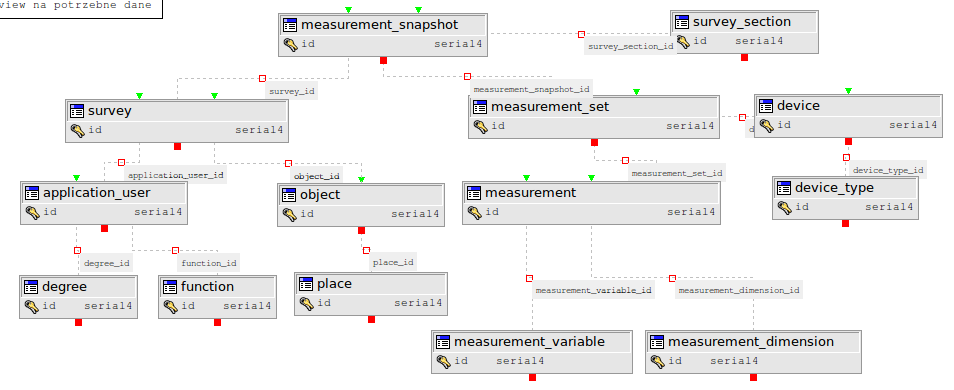
\includegraphics[width=0.95\textwidth]{images/database} 
\caption{Schemat bazy danych} 
\label{template}
 \end{figure} %
\lstset{language=VBScript,
        basicstyle=\footnotesize\ttfamily,
        breaklines=true,
        tabsize=2,
        numbers=left,
        numberstyle=\tiny,
        numbersep=7pt,
        showspaces=false,
        keywordstyle=\color{Blue}\textbf,
        commentstyle=\color{Red}\emph,
        showstringspaces=false,
        stringstyle=\color{BurntOrange}
        }
\section{Instrukcja użytkownika}
%\subsection{Specyfikacja zewnętrzna}
Zaimplementowana przez autora wizualizacja ma na~celu zobrazowanie działania modelu oraz umożliwienie operatorowi wpływania na~jego działanie. Kolejne podrozdziały zawierają opis specyfikacji zewnętrznej oraz wewnętrznej. Część odnosząca się do specyfikacji zewnętrznej jest skróconą instrukcją obsługi użytkownika. Specyfikacja wewnętrzna jest opisem, jak zostały zrealizowane poszczególne elementy~i~w jaki sposób wizualizacja współpracuje ze~sterownikiem.

Ekrany dostępne w wizualizacji oraz klawisze funkcyjne z nimi związane:
\begin{itemize} 
\item Ekran powitalny - F1,
\item Stan robota - F2,
\item Stan magazynu i testowanie obsługi - F3,
\item Testowanie sterowania ręcznego z pilota podłączonego do sterownika - F4,
\item Testowanie sterowania ręcznego z poziomu wizualizacji - F5,
\item Testowanie sterowania automatycznego - F6.
\end{itemize}
\indent
\indent Poszczególne ekrany zostaną szczegółowo opisane w kolejnych podrozdziałach.

\begin{figure}[!htb] 	\centering 	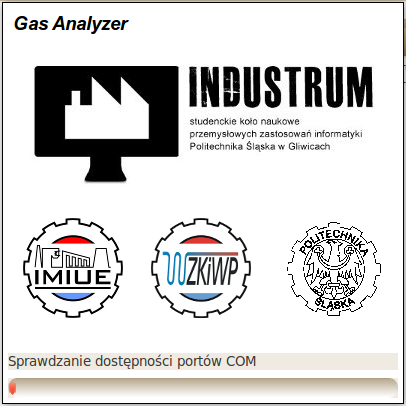
\includegraphics[width=0.5\textwidth]{images/splashScreen.png} \caption{Okno ładowania} \label{template} \end{figure}

\subsubsection{Ekran powitalny}
Bezpośrednio po~uruchomieniu wizualizacji użytkownik zobaczy ekran powitalny taki jak na Rysunku~\ref{vis1} zawierający informacje o~autorze projektu, osobie kierującej projektem (promotorze) oraz informację o~przeznaczeniu wizualizacji wraz ze~zdjęciem modelu. Dodatkowo na~ekranie tym umieszczony został zegar analogowy i~cyfrowy oraz aktualna data.
\begin{figure}[!htb]
\centering 		
  \subfloat[Windows]{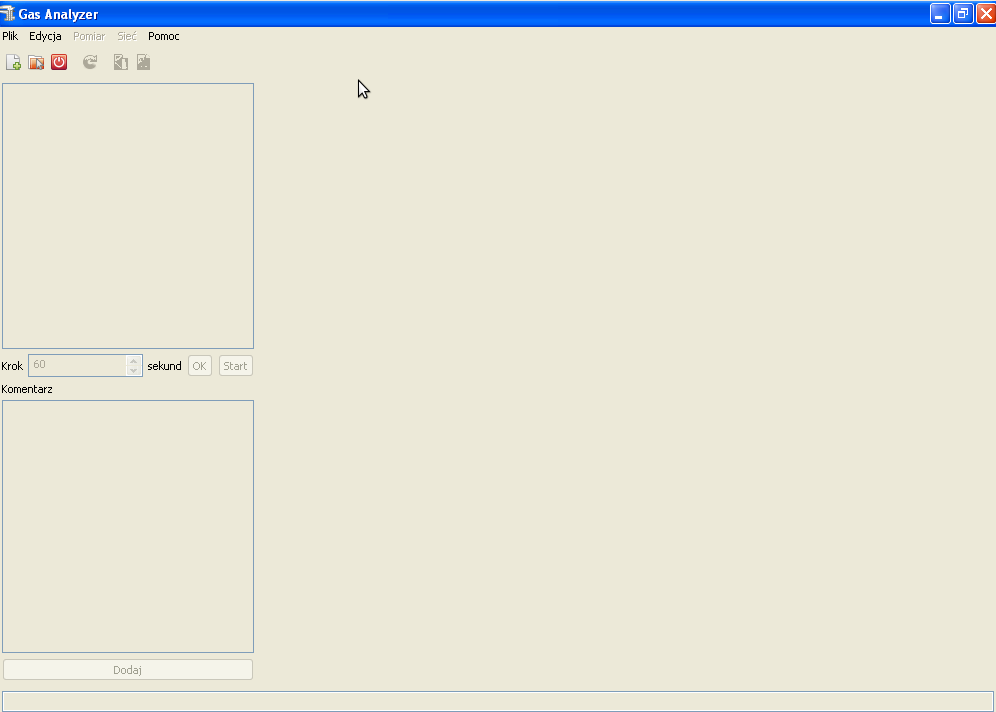
\includegraphics[width=0.45\textwidth]{images/mainW.png}}                
  \subfloat[Linux]{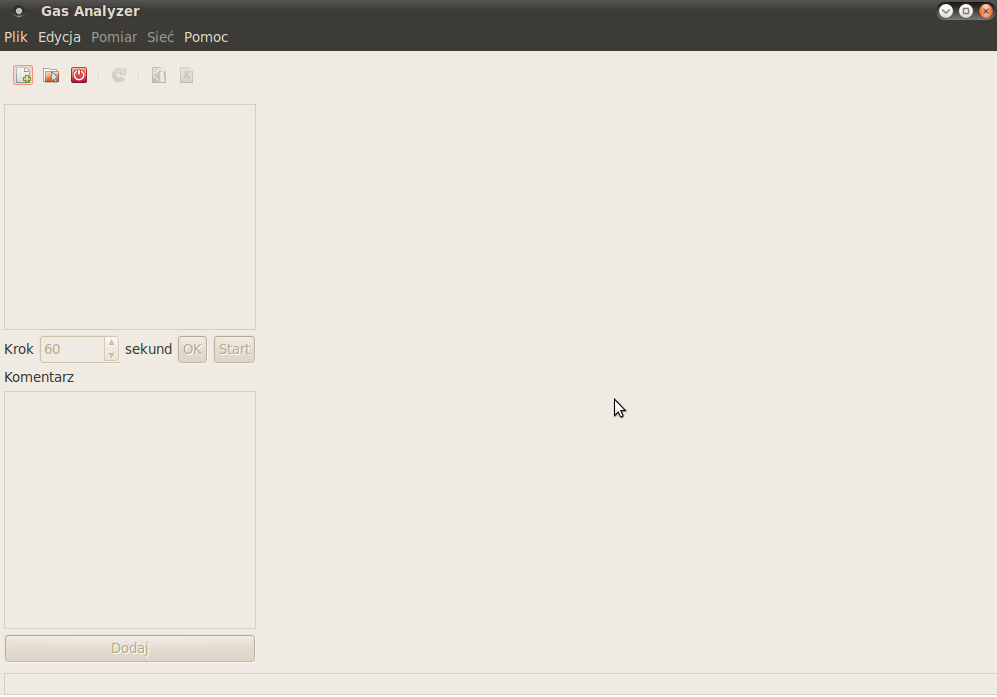
\includegraphics[width=0.45\textwidth]{images/mainL.png}}
\caption{Okno główne} 	
\label{vis1}
\end{figure} %
\section{Podsumowanie}

\subsection{Perspektywy rozwoju}
Projekt jest bardzo perspektywiczny głównie dlatego, że w bieżącej części została zaimplementowana tylko znikoma część protokołu ELAN, a co za tym idzie można cały proces pomiarowy uskutecznić, uprościć oraz zautomatyzować w jeszcze większym stopniu.

\subsection{Wnioski}
Głównymi celami pracy było napisanie oprogramowania gromadzącego dane z urządzeń pomiarowych. %
\section{Bibliografia}
Literatura, która została wykorzystana przez autorów w czasie powstawania projektu, którą opisuje niniejsza dokumentacja.

\begin{thebibliography}{9}
%\begin{enumerate}
%\item 
\bibitem{plc1} 
Jerzy Kasprzyk: 
\emph{"Programowanie sterowników przemysłowych"},
Wydawnictwa Naukowo-Techniczne WNT, 
Warszawa, 
2007      

\bibitem{elan} 
Dokumentacja producenta: 
\emph{„ELAN Interface Description”}, 
sierpień 2006

\bibitem{kurs1} 
Materiały szkoleniowe:
„SIMATIC S7 - Kurs podstawowy”

\end{thebibliography} %
\section{Spis rysunków, tablic i kodów źródłowych}
\subsection{Spis rysunków}
%\listoffigures
\renewcommand*\numberline[1]{Rysunek\,#1:\indent}
\listoffigures
\subsection{Spis tablic}
\renewcommand*\numberline[1]{Tablica\,#1:\indent}
\listoftables
\subsection{Spis kodów źródłowych}
\renewcommand*\numberline[1]{Kod źródłowy\,#1:\indent}
\lstlistoflistings
\section{Załączniki}
\begin{itemize}
\item Płyta CD, na której znajdują się:
\begin{itemize}
\item Pliki wykonywalne w wersji dla:
\begin{itemize}
\item win32 -- Windows 32-bitowy
\item win64 -- Windows 64-bitowy 
\item lin32 -- Linux 32-bitowy
\item lin64 -- Linux 64-bitowy
\item mac32 -- Mac OSX Cocoa 32-bitowy
\item mac64 -- Mac OSX Cocoa 64-bitowy,
\end{itemize}
\item Skrypt tworzący bazę danych,
\item Pliki instalacyjne niezbędne do uruchomienia projektu,
\item Biblioteka RXTX.
\end{itemize}
\end{itemize}
 %

\end{document}
